\documentclass{article}
\usepackage[utf8]{inputenc}
\usepackage{amsmath}
\usepackage{tcolorbox}
\usepackage{amssymb}
\usepackage{amsthm}
\usepackage[
top    = 2.50cm,
bottom = 2.50cm,
left   = 2.75cm,
right  = 2.75cm]{geometry}
\usepackage{fancyhdr}
\pagestyle{fancy}
\lhead{Linear algebra basics}
\rhead{EPFL/Alp Ozen}

\newtheorem{thm}{Theorem}[subsection]
\newtheorem{property}{Property}
\newtheorem{cor}{Corollary}[subsection]

\title{Linear Algebra 1}
\author{alp.ozen}
\date{September 2019}


\begin{document}

\maketitle

\section{Linear equations}
\subsection{Basics}

\begin{tcolorbox}
A linear equation is any equation of form:
$a_{1}x_{1}+ ..... + a_{n}x_{n} = b$
where the a are 'scalars' that belong to a field and the x belong to the vector set. 
\end{tcolorbox}

A \textit{system of linear equation}s is simply a collection of linear equations. The solution of this system, if there is any, is an ordered list $(s_{1},...,s_{n})$ where each $s_{i}$ is the value of each $x_{i}$.
\\

A system consisting of 2 unknowns and two linear equations is generally the intersection of two lines on a cartesian plane. Note that the lines may be parallel or even colinear. 
\\

In general, a system will have:
\begin{itemize}
    \item no solution
    \item unique solution
    \item infinite solutions 
\end{itemize}
\\

We may choose to represent a system of linear equations as an \textit{augmented matrix}. A matrix is called n$\times$m if it is of form:
\begin{equation*}
    \begin{bmatrix}
    a_{11} && a{12} &&  ... \\
    a_{21} && a {22}  && ... \\
    \end{bmatrix}
\end{equation*}

\subsection{Solving a linear system}
\subsubsection{Basics}

When solving a system, our goal is to replace each linear equation with an equivalent set(one that has the same solution) and obtain single linear equations which are trivial to solve. 
\\

In solving a system, we use the elementary row operations which are: 

\begin{tcolorbox}
\begin{itemize}
    \item Interchange two rows (or columns).
    \item Multiply each element in a row (or column) by a non-zero number.
    \item Multiply a row (or column) by a non-zero number and add the result to another row (or column).
\end{itemize}
\end{tcolorbox}

Our goal is to transform our matrix into echelon or row reduced echelon form. A matrix is in echelon form if it looks like this: \begin{equation*}
\begin{bmatrix}
    \blacktriangledown &&  \blacktriangle && \blacktriangle \\
    0 && \blacktriangledown && \blacktriangle \\
    0 && 0 && \blacktriangledown

\end{bmatrix}
    
\end{equation*}

Here, each $\blacktriangledown$ and $\blacktriangle$ may take on any value from the set the vector space is defined on. 
\\

To obtain this form, we first arrange our matrix into a form where the row with the least amount of trailing zeros is placed uptop. Then we ensure the \textit{pivot position}(meaning first non-zero entry) has only 0 in its own column. When done, we move on the second row, find the pivot position and repeat. We repeat this process for all rows. 
\\

If we have a system where the number of unknowns exceeds the number of equations, we obtain a parametric solution. Consider this: 

\begin{example}
\begin{equation*}
  \begin{bmatrix}
    1 && 0 &&  -5 && 1 \\
    0 && 1 && 1 && 4 \\
    0 && 0  && 0 && 0 \\
    \end{bmatrix}
\end{equation*}

Which means: 
$$ x_{1} - 5x_{3} = 1$$
$$ x_{2} +  x_{3} = 4$$

Now, we can express both $x_{1}$ and $x_{2}$ in terms of $x_{3}$. We call $x_{1}$ and $x_{2}$ basic variables and $x_{3}$ the free variable. We call $x_{3}$ a free variable as we are free to choose any value for it. 
\end{example}

Most importantly, these are the conditions for row echelon and reduced row echelon form. 

\begin{tcolorbox}
 \textbf{Row echelon form if:}
 \begin{itemize}
     \item all nonzero rows are above zero rows
     \item a leading entry is the right column of a leading entry above it
     \item all entries in a column below a leading entry are 0
 \end{itemize}
 \textbf{Reduced row echelon also if:}
 \begin{itemize}
     \item leading entry in each nonzero row is 1
     \item the entries in the column of the leading entry are 0
 \end{itemize}
\end{tcolorbox}
\\ 

To obtain reduced row echelon form, starting from the lowest row, the terms in the column with the leading term are made zero and the leading term scaled to 1. We repeat this process. 
\\

As a general remark, we obtain the following.

\begin{thm}
A system is consistent iff, the rightmost column has no pivot. More simply, iff the lowest row is not of the form: 
\begin{bmatrix}
    0 && 0 \dots && b
\end{bmatrix}
where b is nonzero. 
\end{thm}
\\

A common confusion when solving a linear system is why the Gaussian algorithm works? To help answer this, the idea is to visualize a Cartesian plane with two random lines intersecting. Now, there can be multiple lines that intersect at the same point. But the intersection of something like $x=2$ and $y=5$ is obviously $(2,5)$ and requires less effort to solve. Thus, we try to replace our equations with those that are easier to solve and have the same solution set. 

\begin{figure}[h]
    \centering
    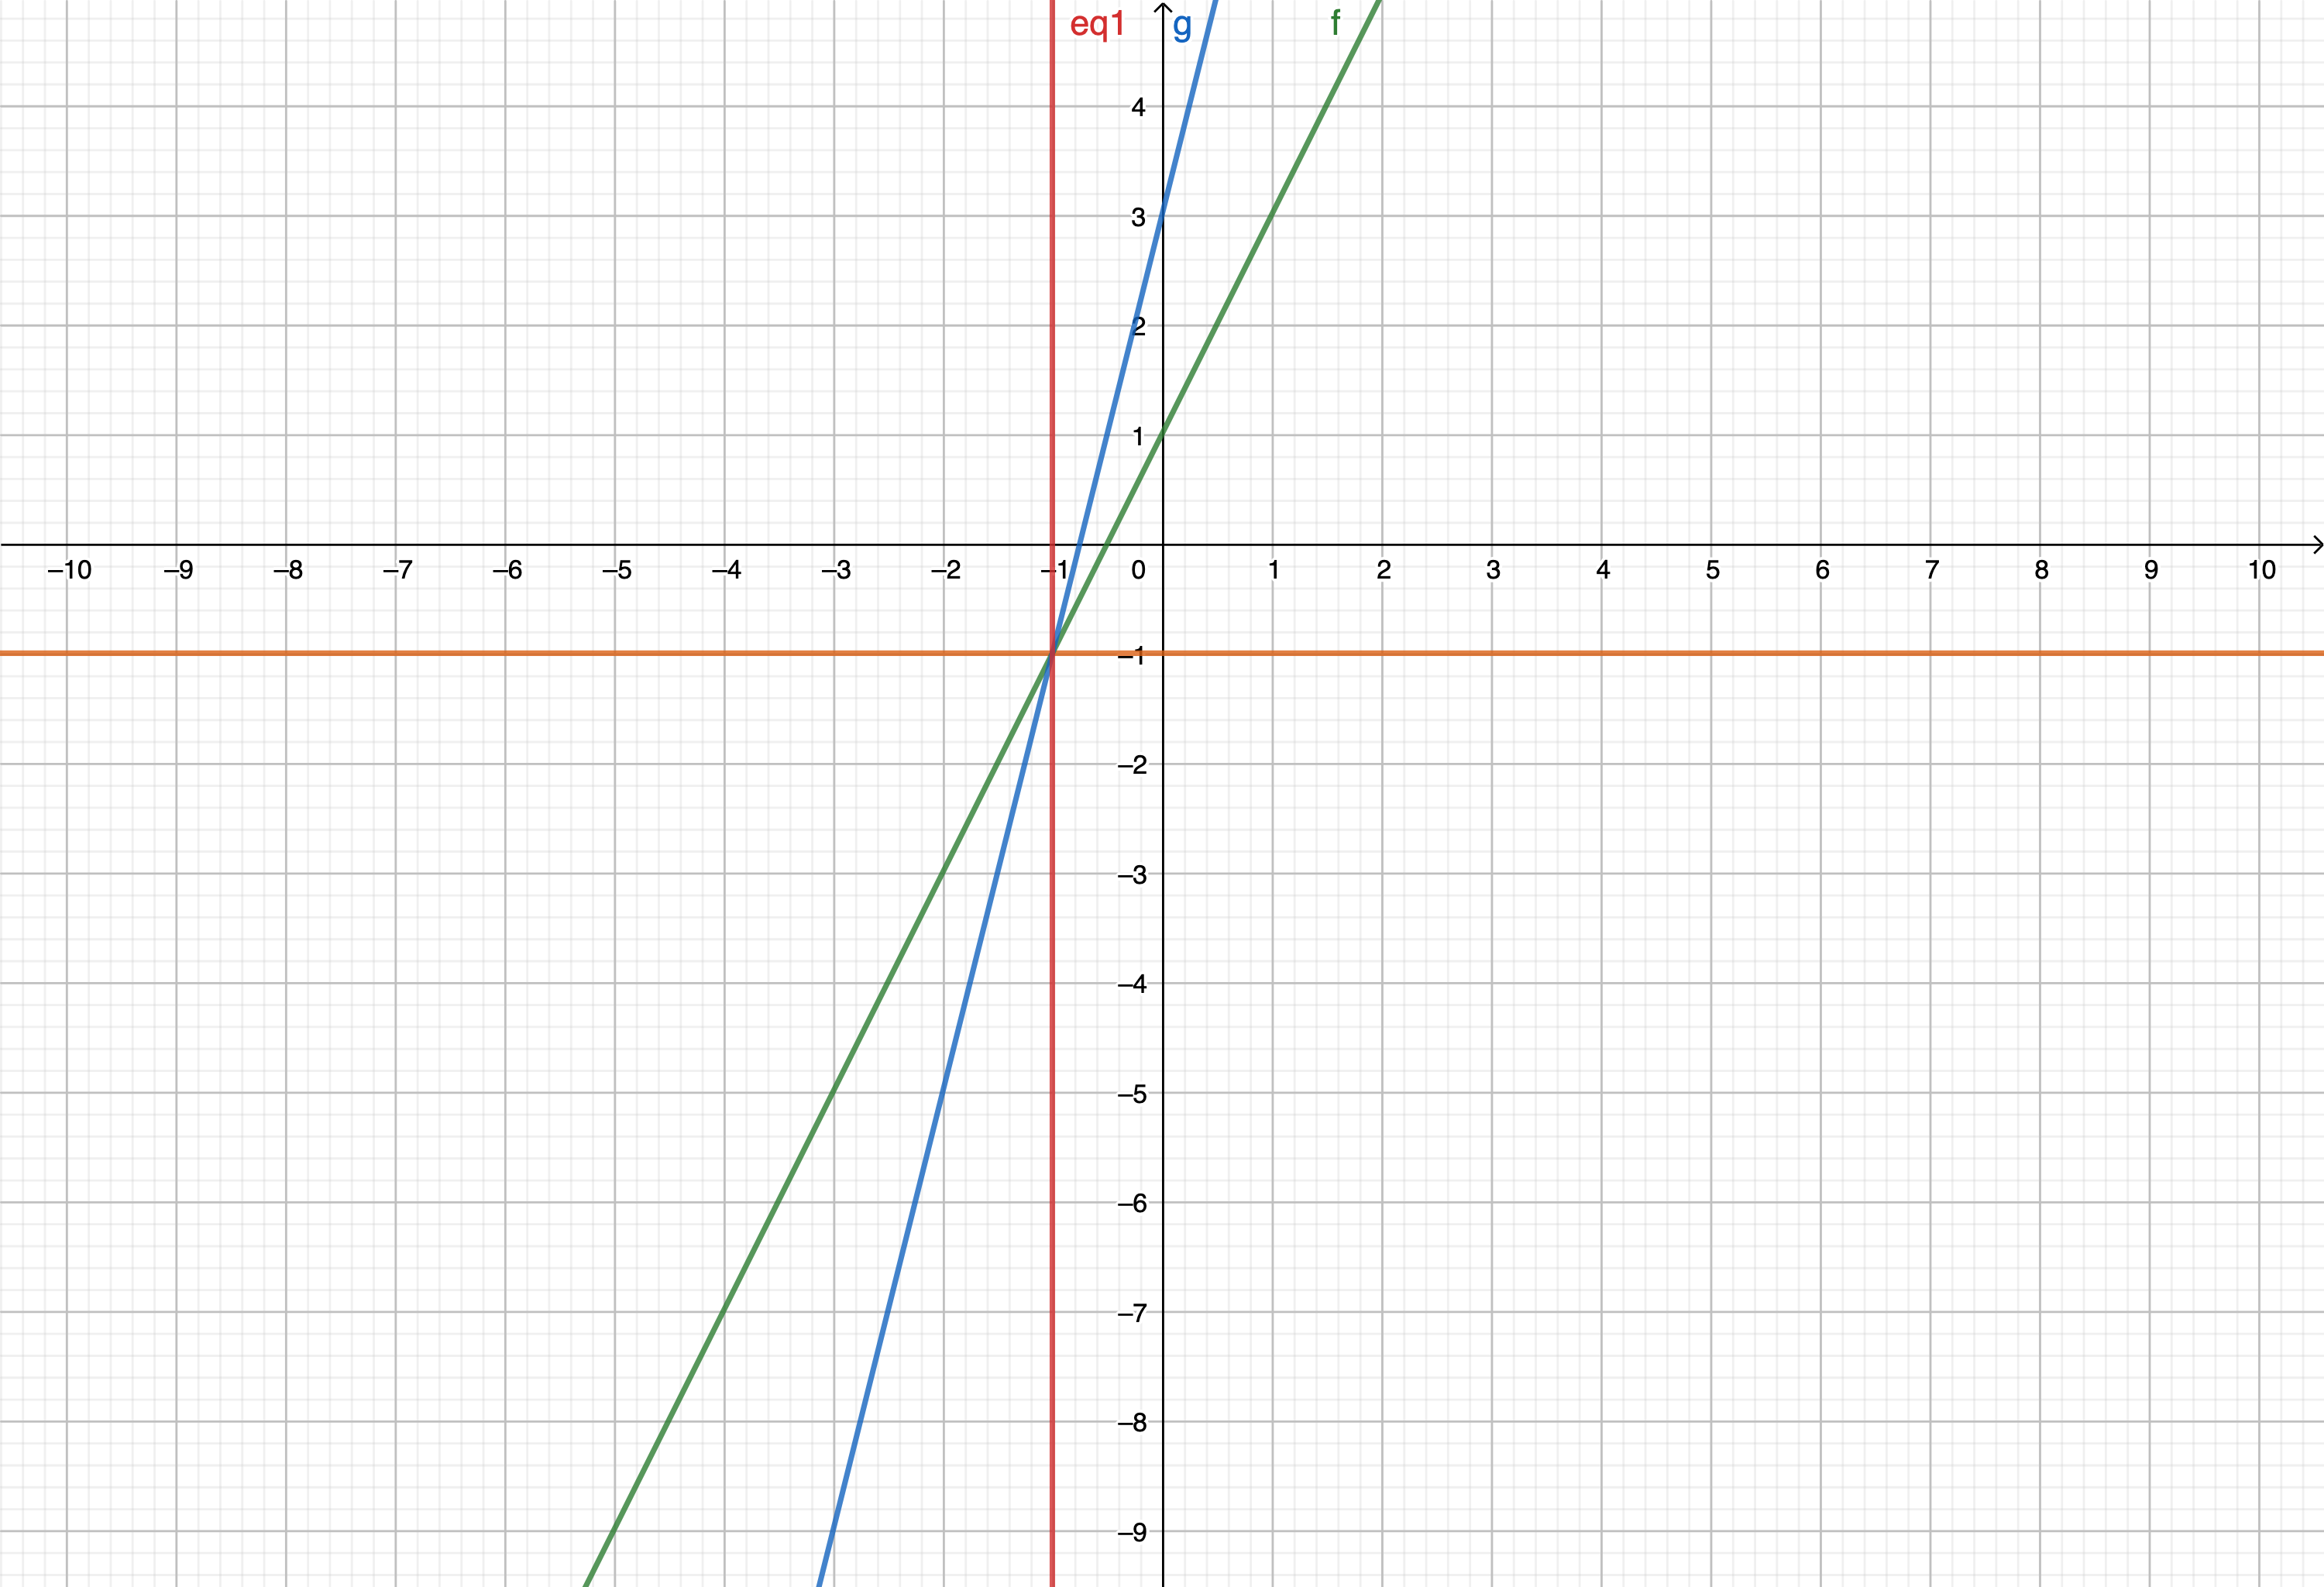
\includegraphics[scale=0.5]{epflSemesterOne/linearAlgebra/figures/linearGauss.png}
    \caption{Equivalent systems}
    \label{fig1}
\end{figure}

\subsubsection{Reducing a system to reduced row echelon form}

\begin{tcolorbox}
    \begin{align*}
     \text{Given} \left(\begin{matrix}0&3&-6&6&4&-5\\3&-7&8&-5&8&9\\3&-9&12&-9&6&15\end{matrix}\right)\\
     \text{We first realign to get} \left(\begin{matrix}3&-7&8&-5&8&9\\3&-9&12&-9&6&15\\0&3&-6&6&4&-5\end{matrix}\right) \\
     \text{After applying elementary row operations, we get the reduced row echelon form of}\\
     \left(\begin{matrix}1&0&-2&3&0&-24\\0&1&-2&2&0&-7\\0&0&0&0&1&4\end{matrix}\right)\\ 
     \text{Now anything which is not a pivot column is called a free variable.}\\
     x_{5} = 4\\
     x_{2} = 2x_{3} - 2x_{4} - 7\\
     x_{1} = 2x_{3} + 2x_{4} - 24
     \end{align*}
\end{tcolorbox}

\subsubsection{High school basics}

When solving systems of 2 unknowns or 3 unknowns, we simply are considering the system of lines or planes. Sticking to 3 dimensions, let's quickly recall how we obtain the formula's of a line and plane in 3-d. 
\\
A line in 3-d may be desribed in Vector form as:
\begin{equation*}
    l_[1] : \begin{bmatrix}
        A\\
        B\\
        C
    \end{bmatrix}
    + 
    \lambda\begin{bmatrix}
        D\\
        E\\
        F
    \end{bmatrix}
    +
    \psi\begin{bmatrix}
        G\\
        H\\
        I
    \end{bmatrix}
\end{equation*}

or may be simplified to cartesian form as: 
\begin{equation*}
    k = \frac{x + A}{B} = \ldots
\end{equation*}

Now, the equation of a plane is most commonly written in the form: 

\begin{equation*}
    Ax + By + Cz \ \text{where (A,B,C) is the normal vector to the plane.}
\end{equation*}

\section{Introducing vector spaces}
\subsection{Basics}
A vector space is an algebraic structure consisting of two sets, a scalar set and the vector set. The scalar set happens to be field and the vector set an additive abelian group. We also define a 'scalar multiplication' between the scalars and vectors to satisfy the following:

\begin{itemize}
    \item $r_{1}r_{2}(v_{1}) = (r_{1}r_{2})v_{1}$  \textbf{associativity of scalar multiplication}
    \item $r_{1}(v_{1}+v_{2}) = r_{1}v_{1}+ r_{1}v_{2}$ and the opposite as well, thus multiplication distributes over addition.
    \item $1_{r}v_{1} = v_{1}$
\end{itemize}

\begin{property}
From the above properties, we can neatly deduce also that $0_{r}v_{1} = 0$
\begin{align*}
    0_{r}v_{1} = (1-1)v_{1}\\
    1v_{1} - 1v_{1} = 0
\end{align*}
\end{property}
\\
The most common vector space is that of $\mathbb{R}^{n}$. It's vector and scalar set are the same. 
\subsection{Linear combinations,span and matrix theorems}

\begin{tcolorbox}
  A \textbf{linear combination} of vectors is simply a sum of vectors multiplied by scalars. 
  \begin{equation*}
      v_{i} = a_{1}v_{1} + \ldots + a_{k}v_{k}
  \end{equation*}
  A \textbf{span} for given vector set $\{v_{1}\ldots v_{k}\}$is simply a set that consists of all the possible outputs of $\sum_{i=1}^{k} a_{i}v_{i}$
\end{tcolorbox}

A common idea in linear algebra is to view a linear combination as the product of two matrices. We can't help but notice that:

\begin{equation*}
    a_{1}v_{1} + \ldots + a_{k}v_{k} = \begin{bmatrix}
        v_{1}  \ldots v_{k}
    \end{bmatrix} \begin{bmatrix}
        a_{1} \\
        \vdots \\
        a_{k}
    \end{bmatrix}
\end{equation*}

An important theorem that follows from the fact that $Ax=b$ is a set of equivalent statements(meaning they always have the same truth value.) 

\begin{thm}
\text{The following are equivalent:}
\begin{enumerate}
    \item $\forall b \in \mathbb{R}^{m}, Ax=b$ \text{has a solution}
    \item $ \forall b \in \mathbb{R}^{m}$ \text{b is a linear combination of the columns of A.}
    \item \text{columns of A span} $\mathbb{R}^{m}$
    \item \text{A(the coefficient matrix!) has a pivot position in each row. }
\end{enumerate}
\end{thm}

\subsection{Homogeneous system of equations}

Any system of linear equations that can be written of the form $Ax = 0$ is called \textbf{Homogeneous}. Clearly, this system has at least one solution which is when x is equal to the 0 vector. The non-trivial solution is if $x$ is not equal to 0 in which case the solution is described in terms of a parameter. Now, a theorem that follows is, for a non-homogeneous system $Ax=b$ with solution $p$, the solution set of $Ax=b$ is the set of vectors of the form $w = p + v_{h}$ where $v_{h}$ is any solution to $Ax = 0$.
\\ We now list some useful theorems. 
\begin{thm}
A homogeneous equation $Ax = 0$ has a nontrivial solution iff it has at least one free variable.
\end{thm}

\begin{thm}
Columns of A are linearly dependent iff $Ax=0$ has a trivial solution.
\end{thm}

\begin{thm}
Suppose the equation $Ax=b$ has a solution p. Then the set of possible solutions to $Ax=b$ are of the form $w = p + v_{h}$ where $v_{h}$ is a solution of $Ax = 0$.(Ofcourse assuming $Ax=b$ is consistent) That is to say, if we knew two solutions to $Ax=b$, we could find a solution to $Ax=0$. 
\end{thm}


\subsection{Linear Independence}
A set of vectors is linearly independent if the solution to:

\begin{equation*}
    a_{1}v_{1} + \ldots + a_{k}v_{k} = 0
\end{equation*}

is only the trivial solution, that is the $0_{v} \in \mathbb{R}^{k}$.
\\
We now present some common statements concerning linear independence. 
\begin{tcolorbox}
  \begin{thm}
    Whenever $Ax=0$ has a nontrivial solution, the columns of $A$ are linearly dependent. 
    \end{thm}
    
    \begin{thm}
    A set of vectors is linearly dependent if at least one of the vectors is a scalar multiple of the other.
    \end{thm}
    
    \begin{thm}
    If a set contains the zero vector, then it is linearly dependent.
    \end{thm}
    
    \begin{thm}
    If a set of vectors contain more vectors than vector entries, the set is linearly dependent.
    \end{thm}
    
    \begin{thm}
    A set of vectors is linearly dependent if the row echelon form of A to $Ax=0$ has at least one free variable.
    \end{thm}
    
\begin{thm}
\label{comb}
A set of vectors is linearly dependent iff at least one of the vectors can be written as a linear combination of the others.
\end{thm}

\begin{cor}
Two vectors are linearly dependent iff one is a scalar multiple of the other
\end{cor}

\end{tcolorbox}
Let's now prove the most useful out of these theorems. 

\begin{proof}
Let's first prove \ref{comb}.
\\
($\rightarrow$)
   Now suppose that for $S = \{ v_{1}, \ldots , v_{k}\}, v_{1} = a_{2}v_{2} + \ldots a_{k}v_{k}$ Then:
   $$ 0 = a_{2}v_{2} + \ldots - v_{1}$$
   In which case $v_{1}$ has a nonzero coefficient implying a nontrivial solution. 
   \\
($\leftarrow$)
Let $j$ represent the vectors that have a nonzero coefficient in $a_{1}v_{1} + \ldots + a_{j}v_{j} + \ldots a_{k}v_{k}$
\\
Now, WLOG, we get for all subscripts less than or equal to $j$:

$$ v_{1} = - \frac{a_{2}}{a_{1}}v_{2} - \ldots - \frac{a_{k}}{a_{1}}v_{k}$$
    \tag*{\qedhere}
\end{proof}

\subsection{Lec 05 notes}

\begin{property}
A linear $T$ maps linear line segments in $\mathbb{R}^{n}$ to linear line segments in $\mathbb{R}^{m}$ 
\end{property}

\subsubsection{Matrix transformations}

\begin{tcolorbox}
  In general, the columns of a matrix are the dimensions of the domain set and the rows of the matrix are the codomain. 
\end{tcolorbox}

























\end{document}